\chapter{Experiments}
\label{chap:experiments}
In this chapter, we elaborate on the dataset used with our model, how we fine-tuned our parameters and the different metrics and method we used to evaluate our solution. We then introduce both qualitative and quantitative results and discuss them.

\section{Experimental protocol}
\label{section:protocol}
In this section, we describe our experimental protocol and introduce the evaluation methods we use.

\subsection{Datasets}
As detailed in chapter \ref{chap:archi}, we use two distinct datasets for our action recognition process. The first one serves as input to the original SOINN model and use preprocessed human body pose estimation frames as input. The body pose estimation is given by OpenPose, but we needed to define a good dataset from which we extract these poses. After a few surveys, we chose to use Hollywood in Homes (HiH) \cite{HiH}. It is a crowdsourced dataset with the following characteristics:

\begin{itemize}
    \item{Composed of 9846 unlabeled videos filmed at 30 frames per second.}
    \item{Average length for each video: 25 seconds.}
    \item{Videos describe everyday indoor scenes in private housing.}
    \item{Typically recorded using smartphone, providing an amateur look that approach typical 2D robot vision perspective.}
    \item{Extremely diverse in terms of subjects, environment, activities, camera angle, lightning conditions, ...}
\end{itemize}
An example of random frames taken from HiH is displayed in figure \ref{fig:HiH}.

\begin{figure}[htp]
\centering
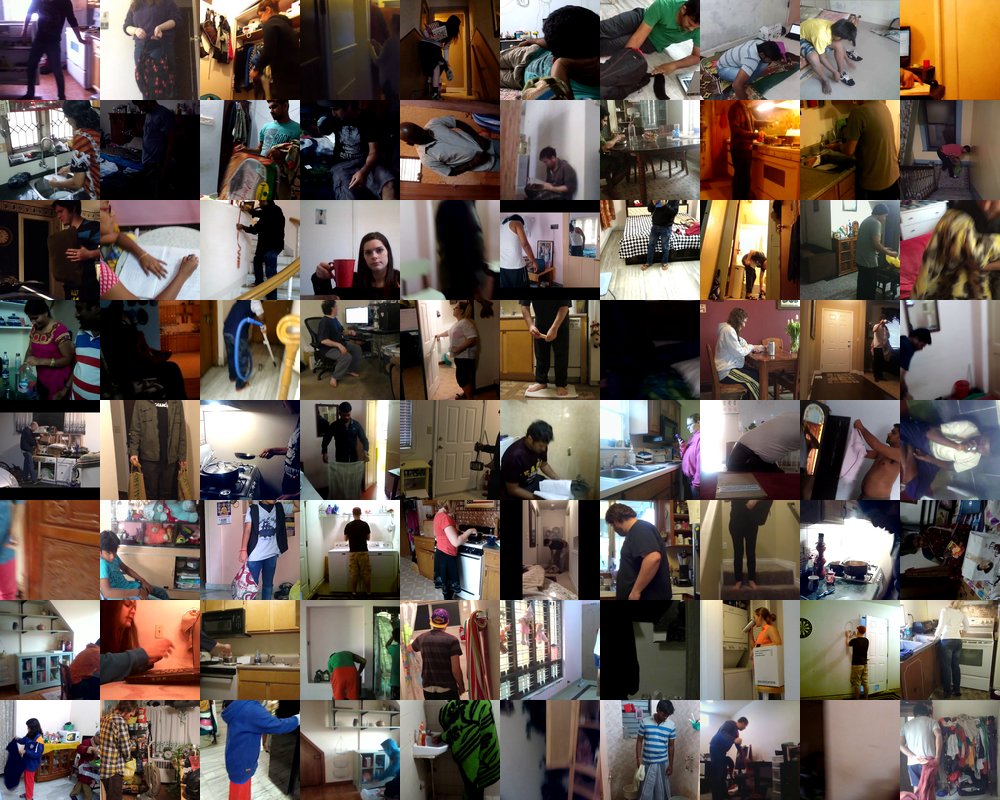
\includegraphics[width=120mm, keepaspectratio]{images/HiH.png}
\caption{Random frames taken from Hollywood in Homes dataset.}
\label{fig:HiH}
\end{figure}

In order to test our method efficiency, we tried its implementation on our turtlebot. We recorded one individual performing a few actions in a small indoor environment: on a 2 minutes long experiment, we record 24 interactions with 6 objects, in an environment of 12 objects including 5 real ones. The 7 others are either one object that has been divided in several parts, or some remaining point clouds from the walls that were not filtered. An example of interaction is displayed in figure \ref{fig:interaction}.

\begin{figure}[htp]
\centering
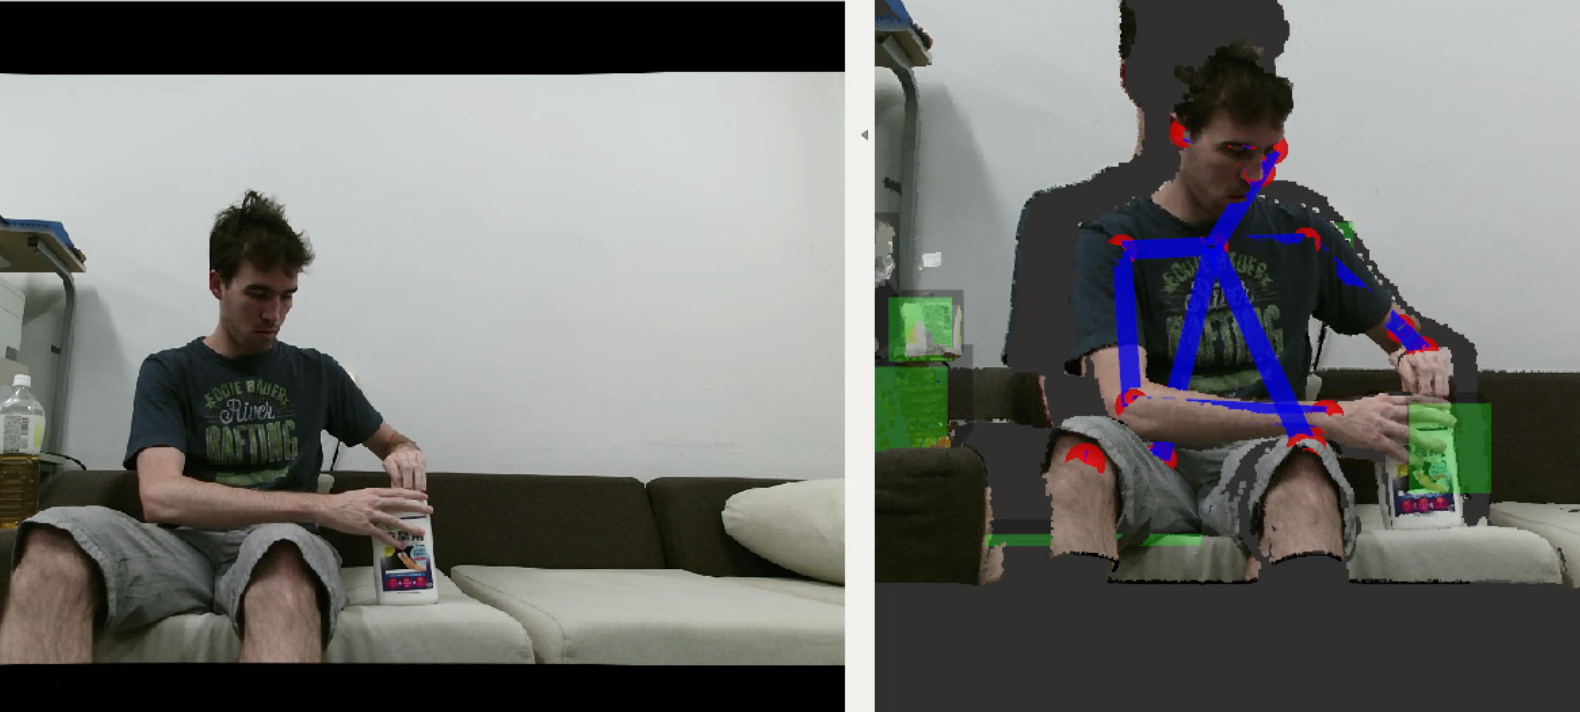
\includegraphics[width=150mm, keepaspectratio]{images/interaction_example.png}
\caption[Example of recorder human/environment interaction]{Example of recorder human/environment interaction. Here, 4 objects are detected: the tissue box we are manipulating, the plastic bottle - that is badly detected as 2 objects due to its transparency, and a part of the couch. Here, two interactions are recorded: one with the couch and one with the tissue box.}
\label{fig:interaction}
\end{figure}

\subsection{Metrics used}
It is often difficult to evaluate an unsupervised clustering algorithm. In supervised classification, a natural metric is average accuracy, where the accuracy is simply the proportion of well classified examples, with examples taken from a labeled dataset where we know the ground truth. For unsupervised clustering, the algorithm separates data in clusters but do not issue a label for these clusters. 

Nevertheless, it is sometimes possible to evaluate them by using a labeled dataset from which we hide the labels to the algorithm during training, and we can then compare the outputs of the algorithm with the ground truth labels by several means. However this type of evaluation technique is only possible if we have labeled data to use. Unfortunately, it is not the case in our study, since our original dataset is unlabeled and our refined algorithm makes use of data that is personal to the robot. 

For these reasons, we only have access to a few metrics that do not involve any ground truth comparison. The first one that can be considered is called the relative size of the model $N_{rel}$. It is simply defined as the number of nodes output by the algorithm divided by the size of the training set for a cluster model C: 

\begin{equation}
    N_{rel}(C) = \frac{|C|}{size_{train}(C)}
\end{equation}

$N_{rel}$ is basically the reduction power of the algorithm, which represents its capacity to summarize its input. However, it gives no indication about the quality of that reduced model.

In order to evaluate this quality, we introduce another classical evaluation metrics: the Sum of Squared Errors (SSE)\cite{sse-silhouette}. SSE is defined by:

\begin{equation}
    SSE(C) = \sum_{i=1}^k\sum_{o \in C_i}d(o, cen_{i})^2
\end{equation}

where C is a cluster model output by the algorithm, composed of k clusters $C_i$, and $cen_i$ is the centroid of cluster $C_i$. SSE basically punishes clusters that are too much spread, it is a good measure complementary to $N_{rel}$.

The last metrics available for data without ground truth is the silhouette measure. The silhouette measure of an object $o_i$ assigned to a cluster $C_A$ is:
\begin{equation}
    sil(o_i)= \frac{b(o_i) - a(o_i)}{max\{a(o_i), b(o_i)\}}
\end{equation}
where $a(o_i)$ represents the average distance between $o_i$ and the other objects in the cluster and $b(o_i)$ is the average distance between $o_i$ and the objects in the nearest cluster:

\begin{equation}
    a(o_i) = \frac{1}{|C_A|-1}\sum_{o_j \in C_A, o_j \neq o_i}d(o_i, o_j)
\end{equation}
\begin{equation}
    b(o_i)= \min_{C_B \neq C_A} \frac{1}{|C_B|} \sum_{o_j \in C_B}d(o_i, o_j)
\end{equation}

From there, we can define the silhouette of a cluster as the average silhouette of its objects:
\begin{equation}
    sil(C_i)=\frac{1}{|C_i|} \sum_{o_j \in C_i}sil(o_j)
\end{equation}

and finally the silhouette of the entire model C:
\begin{equation}
    sil(C)= \frac{1}{k} \sum_{i=1}^k sil(C_i)
\end{equation}

The silhouette measure is interesting since it does not just evaluate the average object/centroid inside distance of each cluster, but mitigates it with the object/centroid distance augmentation if that cluster was to disappear.

\subsection{Parameters fine-tuning}
In this section, we detail the value we chose for the different parameters in our model. We summarize the chosen values in table \ref{tab:parameters}.

The SOINN algorithm itself takes two parameters as input: the period at which it deletes nodes $\lambda$ and the maximum age of a neighbourhood relationship between two nodes $\gamma$. When testing SOINN with human poses as input, we observed little influence of $\lambda$ on the result, and $\gamma$ tends to fuse too much nodes at its standard value of 50, however the number of nodes increased dramatically for $10 < \gamma < 20$ so we set it at 30 to find a good compromise.

The pre-processing part of our workflow impose a quality threshold T on the pose estimation of the dataset to be considered as valid training data. When $T > 70\%$, the training becomes really long since a lot of frames in the dataset are not well-estimated. It also make SOINN produce more nodes since he becomes more selective on the slight differences between inputs. However, this is not a good thing for subsequent clustering with unfiltered data: most of the pose estimation received as real-time input are not that precise: this situation would lead our model to overfit.
However if T is too low, it is almost as if we do not require any minimum quality for input frames, which means that our model would sometimes learn pure artifacts. We observed that a value of 60\% is the best compromise to avoid these issues as much as possible.

Another thing we have to decide for the pre-training part of our workflow is the size of the pre-training set. If the training set is too small, SOINN is not stable enough to handle unfiltered data of lower quality. On the opposite, a too large training set makes the model too rigid and less likely to be influenced by the add of spatial context information. It also reduces the quality of its nodes. We chose to let SOINN learn from 5000 good body pose detection before we make it take unfiltered data as input.

The object detection part of our workflow uses euclidean cluster extraction. This technique requires to specify the expected size of detected object by indication a minimum and maximum number of points that can contain an object. This parameter is extremely dependent on the environment, and may need to be adapted in real-time to control the number of detected objects. On our test environment, we obtained best results at $min_{points}=500$ and $max_{points}=10000$ but it may vary at lot from one environment to another. We also add a tolerance parameter for this model, which defines the distance under which two objects may be fused, in terms of a percentage of the object sizes. It was originally at 0.01, but we raised it to 0.02 to avoid too much outputs consisting of several clouds for one real object.

Finally, our modified SOINN algorithm needs three additional parameters: the bonus and malus used to compute the new distance, and the learning rate $\alpha$. In this work, we chose to set bonus to 0.5 and malus to 2 so that they affect signals in the same way, but that may be tuned better in potential future works. $\alpha$ was added to help the model build confidence in its first inputs. We initially wanted to make it converge to 1 as the model receives more signals, but it did not seem to affect the result so we kept it at its original value of 2.

\begin{table}[hp]
\centering
\caption{Parameters tuning results}
\label{tab:parameters}
\begin{tabular}{|c|c|c|}
    \hline
    Parameters & Value range & Value used \\
    \hline
    $\lambda$ & [50, 200] & 100 \\
    $\gamma$ & [10, 50] & 30 \\
    T & [0.5, 0.8] & 0.6 \\
    $N_{train}$ & [1000, 10 000] & 5000 \\
    tolerance & [0.01, 0.05] & 0.02 \\
    $min_{points}$ & [100, 2000] & 500 \\
    $max_{points}$ & [5000, 100 000] & 10 000 \\
    bonus & [0.1, 0.9] & 0.5 \\
    malus & [1.1, 3.0] & 2.0 \\
    $\alpha$ & [1.0, 5.0] & 2.0 \\
    \hline
\end{tabular}
\end{table}

\subsection{Comparison method}
We begin by pre-training the standard SOINN algorithm on the same subset of our dataset. We take a copy of this model and convert this copy to a context-aware equivalent model that we train using the method described earlier.

Since our algorithm now manipulates [pose, interaction] signals instead of normal pose signal of naive pose estimation, it is difficult to evaluate the performance gain that it brings. In order to compare our proposed modified algorithm with naive pose estimation, we will project the outputs to normal body pose space. By doing that, we can compute scores that we can compare against each other using the metrics described above. 

However, we should keep in mind that these evaluations only partly represent the information gain we get from human/object interaction context to the model, and we can only infer that the unprojected model behaves similarly.

\section{Results}
In this section, we show both visual results and numeric evaluation scores computed using methods described in section \ref{section:protocol}.
\subsection{Results visualization}
We begin by showing the results of classical SOINN algorithm after pre-training on pose only during 5000 frames. We highlighted a few outputs among the 104 output nodes in figure \ref{fig:similar_nodes} to show that some of them depict poses that obviously belong to the same clusters. On the other hand, the context-aware SOINN algorithm we designed outputs less nodes: it transforms the previous 104 nodes to 92 new ones for the same example, which is a good thing if it does not increase the model global error, we will discuss this point in the next part.

It seems that it mainly operated by fusing existing nodes (see figure \ref{fig:nodes_fusion}), but it does not seem that the model separated further the previous nodes in the examples we computed. This is a good behaviour for our examples, since classical SOINN always output an overestimated number of nodes in our cases, so fusing was more necessary than separating, but it is difficult to infer whether or not our algorithm would be able to efficiently separate existing nodes in other applications.

\begin{figure}[htp]
    \centering
    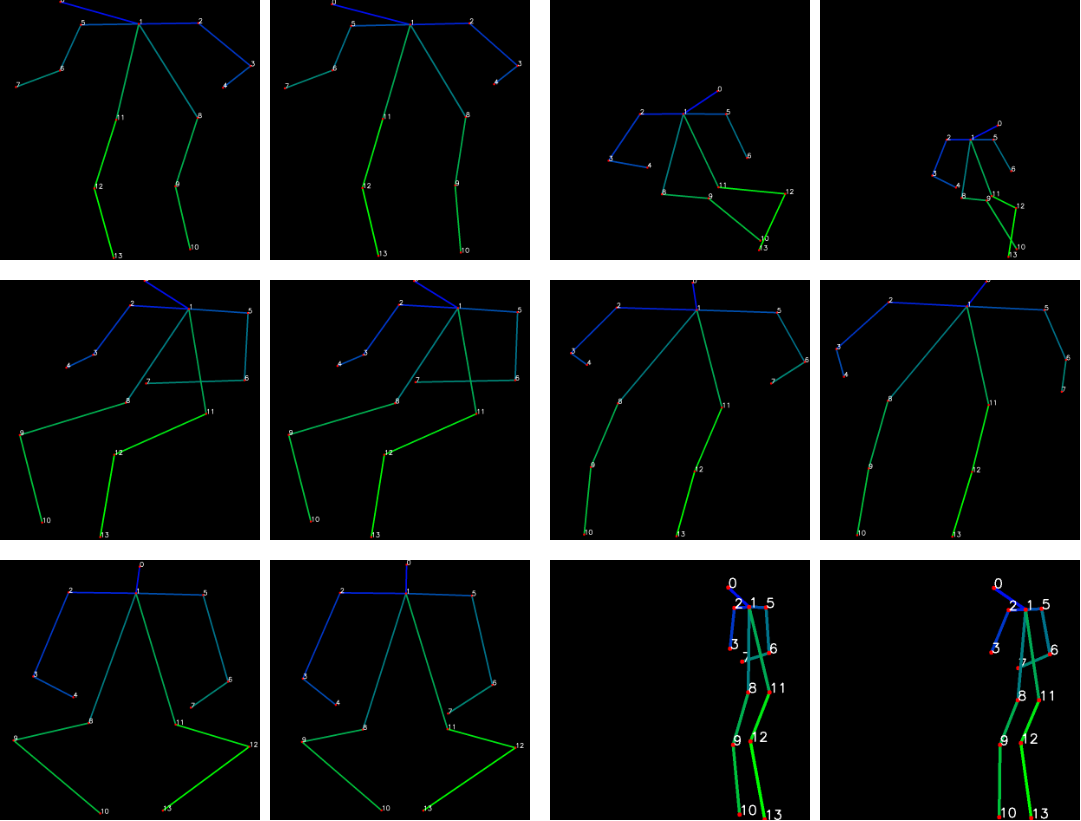
\includegraphics[width=150mm, keepaspectratio]{images/similar_nodes.png}
    \caption[Example of nodes issued by naive algorithm]{Example of nodes issued by naive algorithm. We see the limit of this model as some nodes are very close to each other.}
    \label{fig:similar_nodes}
\end{figure}

\begin{figure}[htp]
    \centering
    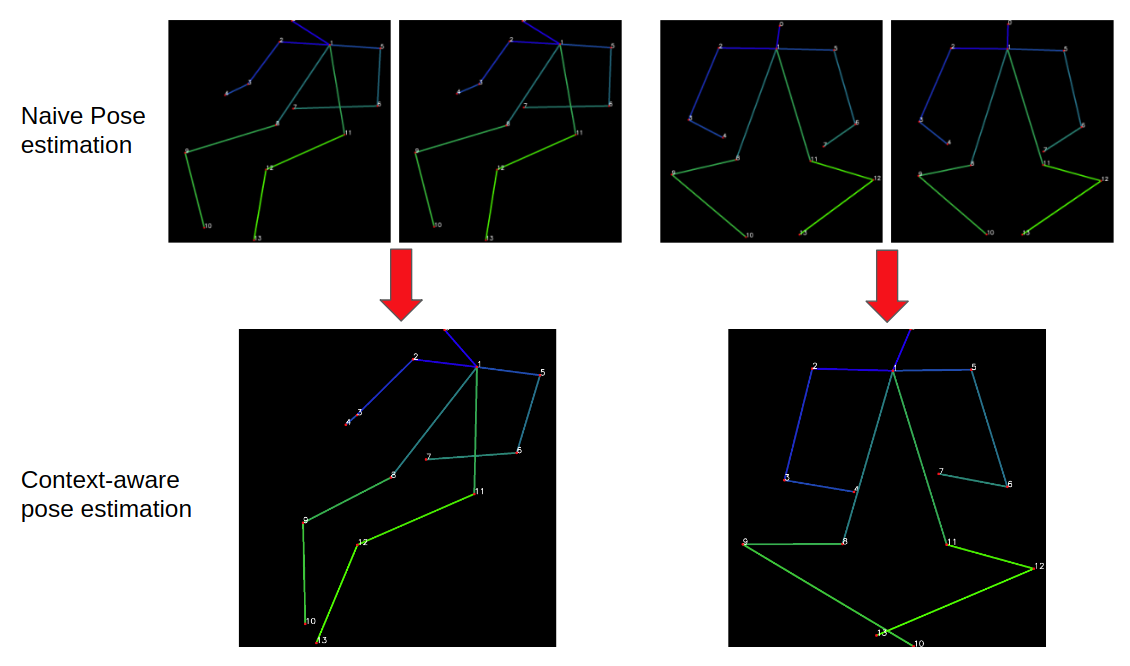
\includegraphics[width=150mm, keepaspectratio]{images/nodes_fusion.png}
    \caption{Example of node fusion operated by our method}
    \label{fig:nodes_fusion}
\end{figure}

\pagebreak
\subsection{Results evaluation}
According to the method described in the previous section, we compute and compare scores obtained by classical SOINN versus context-aware SOINN. The results are displayed in table \ref{tab:SOINN_comp}.

We see on this table that the introduction of spatial context information globally reduces the number of nodes. The refined algorithm performs also slightly better in regard to SSE score, but that difference is less significant when comparing the silhouette of the two models.

However, by analyzing the silhouette profile of each node for both original and refined SOINN models - respectively in figure \ref{fig:silhouette_before} and figure \ref{fig:silhouette_after} - we notice than our model tends to increase the spread of the original nodes score distribution. We can interpret this result by affirming that our model is likely to increase the silhouette score of our model if object detection is well executed and human/object interaction is relevant - as demonstrated by nodes where the score increases locally - but our imperfect current implementation may cause the opposite effect when the context information provided to the model is not relevant.

\begin{table}[htp]
\centering
\caption[Numerical evaluation of our method]{Numerical evaluation of our method. We compare the result of basic SOINN algorithm (in green) and context-aware SOINN (in blue). This result is the average of 10 distinct tests on 100 validation frames.}
\label{tab:SOINN_comp}
\begin{tabular}{|c|c|c|c|c|c|c|}
    \hline
    $N_{train}$ (frames)  & \cellcolor[HTML]{009901}$N_{rel}$ & \cellcolor[HTML]{009901}SSE & \cellcolor[HTML]{009901}silhouette & \cellcolor[HTML]{3166FF}$N_{rel}$ & \cellcolor[HTML]{3166FF}SSE & \cellcolor[HTML]{3166FF}silhouette \\
    \hline
    1000 & 29.41 & 456.14 & 0.45 & 35.71 & 388.20 & 0.46 \\
    2000 & 31.5 & 349.72 & 0.46 & 36.36 & 309.61 & 0.48 \\
    5000 & 48.08 & 190.38 & 0.51 & 54.34 & 175.55 & 0.51 \\
    10000 & 70.42 & 182.70 & 0.51 & 87.47 & 162.27 & 0.53 \\
    \hline
\end{tabular}
\end{table}

\begin{figure}[ht]
    \centering
    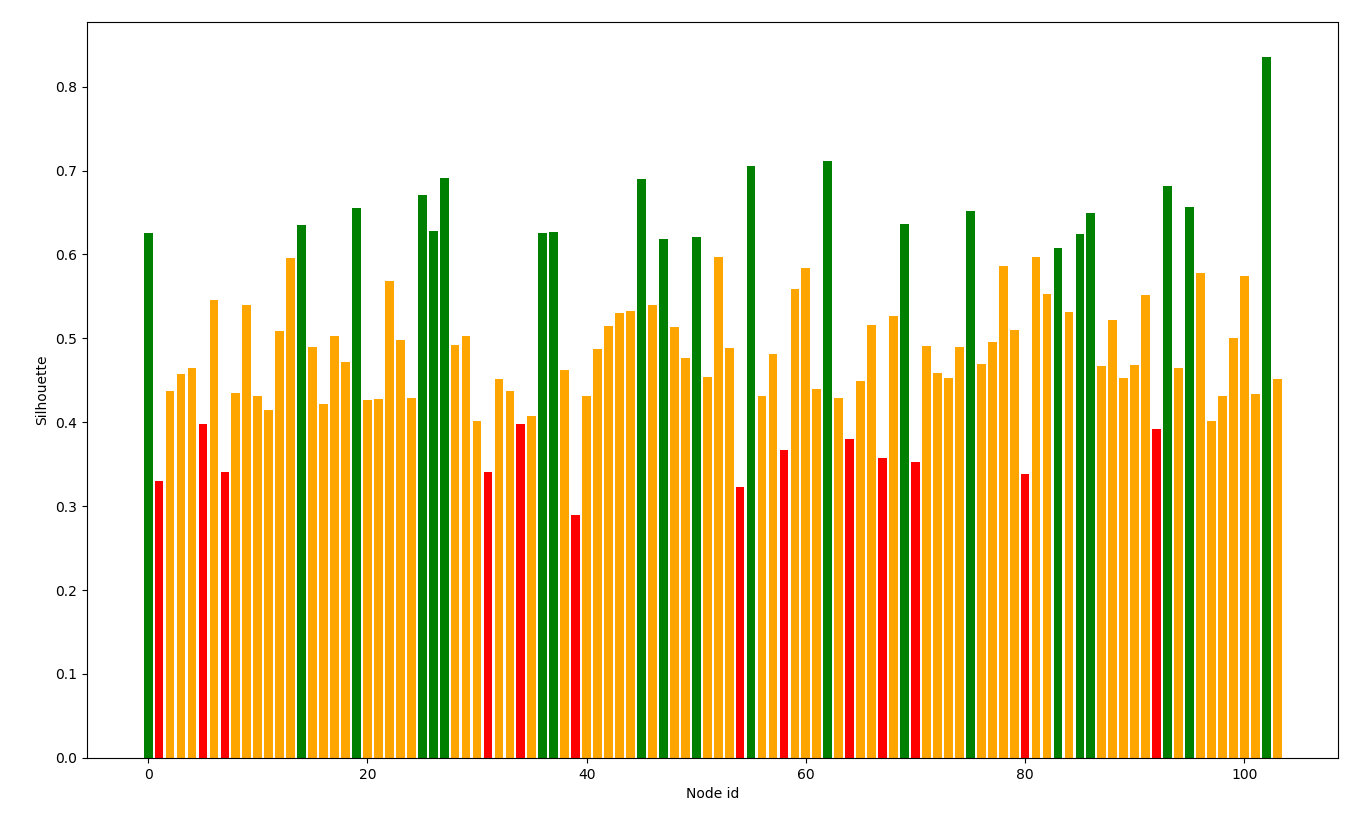
\includegraphics[width=130mm, keepaspectratio]{images/silhouette_original.png}
    \caption[Silhouette score repartition for original SOINN]{Silhouette score repartition for original SOINN, $N_{train} = 5000$. Colors represents three ranges of value: less than 0.4, [0.4, 0.6] and more than 0.6}
    \label{fig:silhouette_before}
\end{figure}

\begin{figure}[ht]
    \centering
    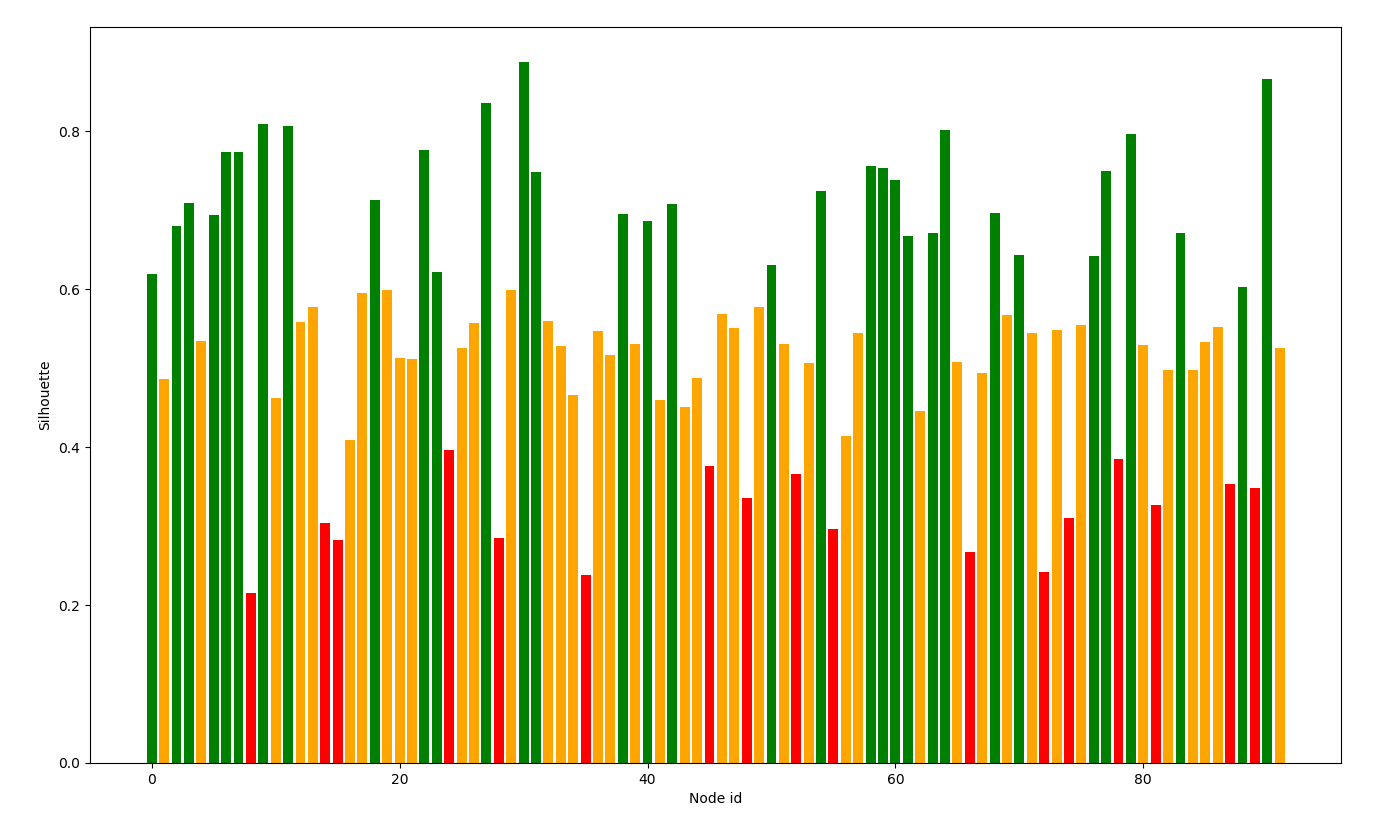
\includegraphics[width=130mm, keepaspectratio]{images/silhouette_refined.png}
    \caption[Silhouette score repartition for spatial context-aware SOINN]{Silhouette score repartition for spatial context-aware SOINN, $N_{train} = 5000$. Colors represents three ranges of value: less than 0.4, [0.4, 0.6] and more than 0.6}
    \label{fig:silhouette_after}
\end{figure}